% !Mode:: "TeX:UTF-8"

\chapter{基于方法间关联关系的代码变更影响分析}

%%%%%%%%%%%%%%%%%%%%%%%%%%%%%%%%%%%%%%%%%%%%%%%%%%%%%%%%%%%%%%%%%%%%%%%%%%%%%%%
\section{引言}

软件变更是软件维护的核心环节。对软件系统的修改可能引发系统其他部分的不良副作用或连锁反应。而变更影响分析的目标在于识别变更的涟漪效应,帮助开发者安全地进行变更。方法之间的变更影响可以分为以下两种类型:

(1)依赖型变更影响关系:依赖型指的是能直接体现在代码静态结构中的变更影响关系,如将项目代码组织为抽象语法树、系统依赖图或影响图,通过图结构的可达性分析,得到方法和方法之间的静态依赖关系。这种依赖型的变更影响关系体现为表现为方法间的调用或间接调用关系。

(2)逻辑型变更影响关系:在这种类型的变更影响关系中,方法之间不存在静态结构之间的关联关系,但它们的实现逻辑或所操作的数据之间存在某种隐含的关联。具体来说,这种关系可能源于它们共同维护某个数据的一致性、共享某些资源,或其功能逻辑有某种预期联系。因此,当某个方法发生变化时,可能会间接影响到其他方法的行为或结果。

依赖型影响关系可在代码的静态结构中直接显现,通过传统静态分析方法甚至开发工具即可捕捉,而逻辑型影响关系通常只能通过开发者人工进行分析提取,正是因为此种关系的存在,导致了开发者对软件代码的维护非常困扰,难以理解软件架构、难以安全变更的问题出现。

为了解决上述问题,本文以C/C++项目为研究对象,实现了基于依赖关系闭包的传统分析方法,并实现了基于依赖关系、基于克隆关系以及基于变更历史和共现关联关系的的变更影响分析方法,从而能够全面挖掘这依赖型和逻辑型的变更影响关系,并通过实验对比分析了这三种方法在提取这两类影响关系的有效性。


\section{代码预处理和中间表示生成}


\subsection{基于clang的抽象语法树生成}
抽象语法树(Abstracted Syntax Tree,AST)是一种用来表现编程语言构造的树状结构,它把代码的语法结构以树形的方式进行了抽象化描述。在这个树形结构中,每一个节点都对应着代码中的某个元素,比如变量声明、语句或者是表达式等。从抽象语法树的根节点出发,代码逐步被拆解成更小的部分,直到最终到达叶节点,这些叶节点代表了代码中最基本的元素,如操作符或变量等。在抽象语法树中,节点之间的连接表明了它们之间的层级关系,即父节点与子节点的关系。通过这样的结构,AST 能够清晰地展示出代码的层次和结构,为编译器或其他工具分析和处理代码提供便利。


Clang 是由苹果公司发起的支持 C、C++、Objective-C 和 Objective-C++语言的编译器前端,负责对代码进行词法分析、语法分析和语义分析,对程序代码的分析和理解至关重要\cite{clang}。词法分析通过识别 Token 将程序代码分解成基本单元。语法分析在此基础上识别程序的语法结构,构造抽象语法树。语义分析消除语义模糊,生成属性信息,让计算机生成目标代码。而libclang 是 Clang 编译器的一个重要组成部分,它提供了一套用于解析源代码的程序接口。这些程序接口允许开发者在项目中使用 Clang 的强大语言解析和代码分析功能\cite{libclang}。本文使用libclang 生成AST ,提取代码中的调用和依赖关系,为后续进一步分析提供基础。


这里通过一个简单的例子来说明libclang的使用方式。如图 2-1 所示,这里定义了一个简单的 C 语言文件,文件中声明并定义了了两个方法和一个全局变量,主函数用于计算两个数的和。

\begin{figure}[h]
\centering
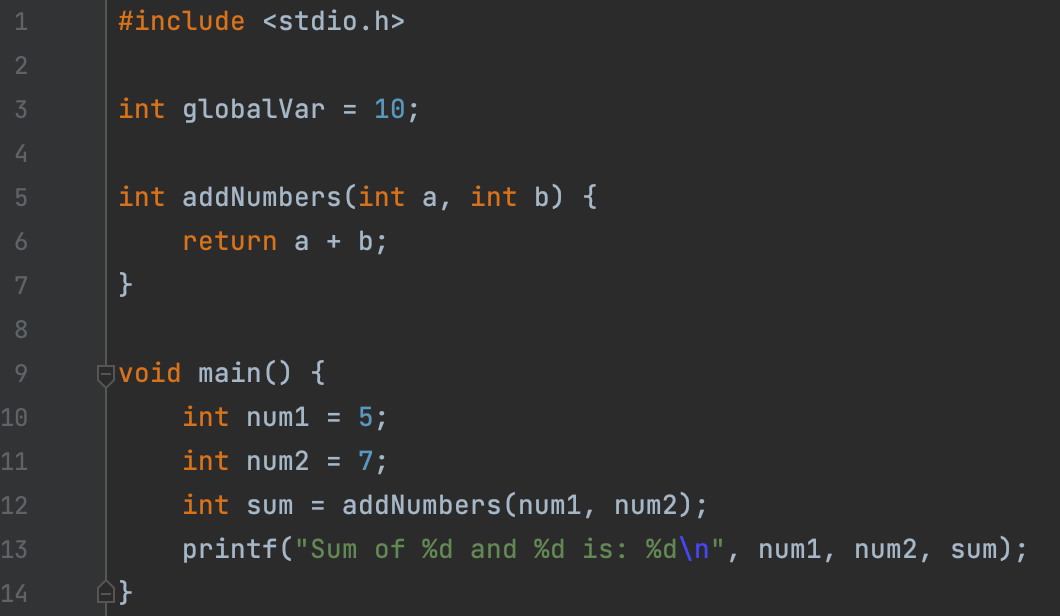
\includegraphics[width = 0.6\textwidth]{代码示例}
\caption{示例代码}
\end{figure}


这段代码由 Clang 解析生成抽象语法树后,得到的树结构如图 2-2 所示。

\begin{figure}[h]
\centering
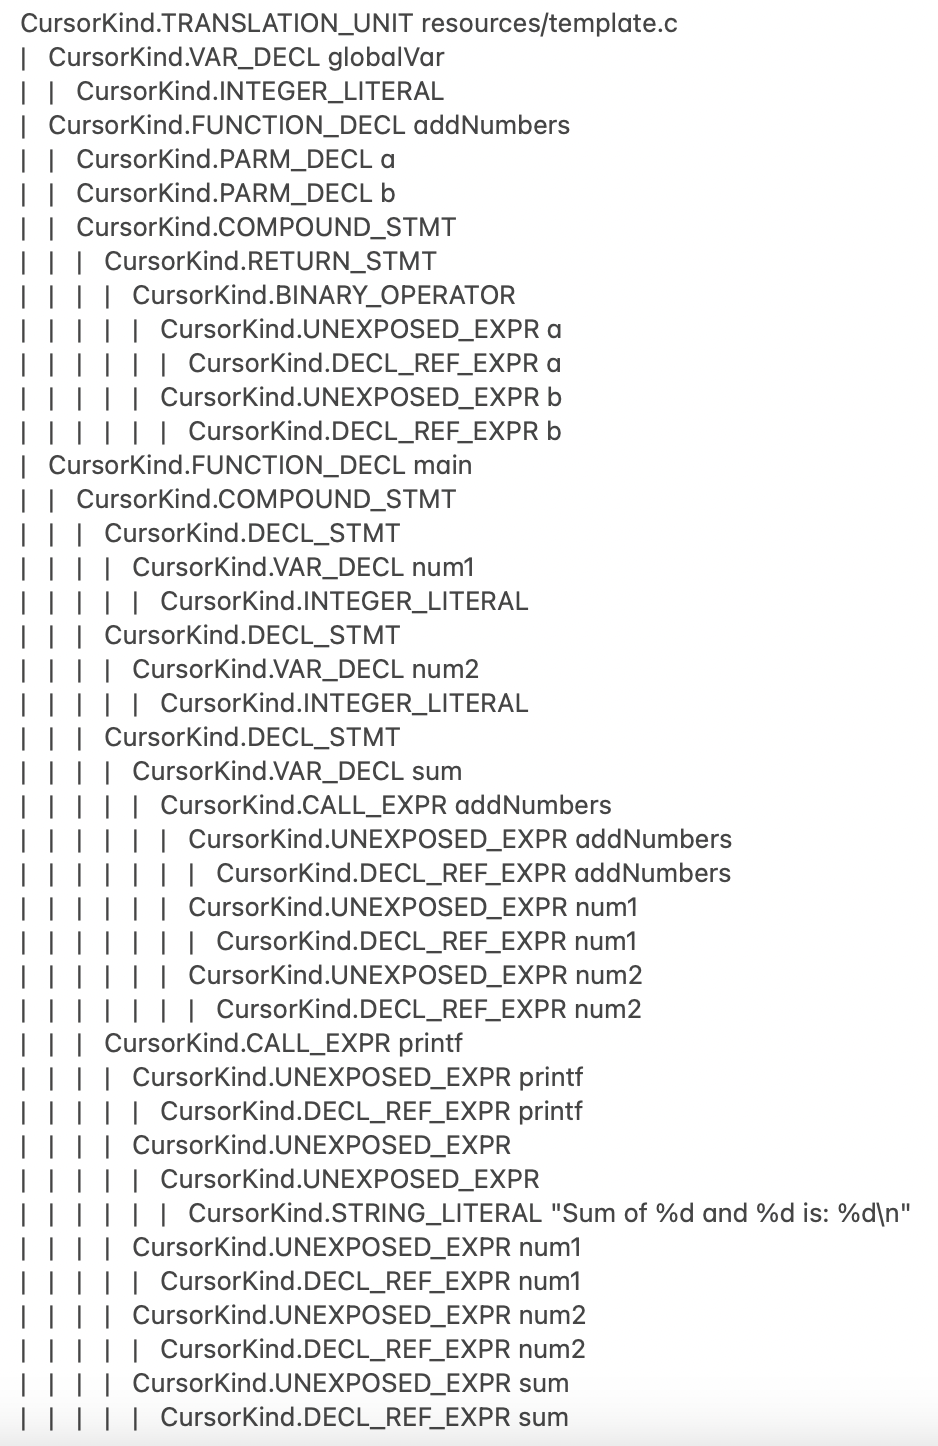
\includegraphics[width = 0.6\textwidth]{ast示例}
\caption{示例代码对应的抽象语法树结构}
\end{figure}

在 libclang 解析得到的抽象语法树中,游标(cursor)是一个核心概念,它作为一个指针或引用存在,每个 cursor 都与 AST 中的一个特定节点相对应,表示了源代码中的一个结构元素。通过操作 cursor,可以遍历整个 AST,访问和分析代码中的各种元素,如获取变量的类型、方法的参数列表、类的成员等。libclang 提供了一系列 API 函数来操作 cursor,例如:遍历 AST 中的 cursor、获取 cursor 的类型(如是否为方法定义、变量定义、变量引用等)、获取 cursor 所代表的源代码元素的名称、类型、位置等信息、获取 cursor 的父节点或子节点等。本文通过操作游标,遍历 AST,获取整个 AST的结构。


Clang 定义了一套节点类型标识。AST 的顶层节点类型是Translation\_Unit标签,表示一个翻译单元,对 AST 树的遍历,实际上就是遍历整个Translation\_Unit。Function\_Decl指的是方法定义,在 clang 中是不区分方法声明和方法定义的,统一用 Function\_Decl来标识,两个区分主要看是否有方法体,在 libclang 中提供了程序接口供开发者调用判断。Parm\_Decl 是参数节点,上面的例子中,方法 addNumbers 有两个参数 a 和 b。CompoundStmt 代表大括号,方法实现、struct、enum、for 的 body 等一般用此标签包起来。DeclStmt 是定义语句,里边可能有 VarDecl 等类型的定义,VarDecl 是对变量的定义。CallExpr 标签表示方法调用 Expr,子节点有调用的参数列表。ReturnStmt 表示返回语句。


\subsection{方法调用链提取与分析}
在使用 libclang 提取代码的抽象语法树后,遍历整棵树来提取方法之间的调用关系。这部分我们重点关注抽象语法树上的方法节点,以及方法节点内部的调用节点,分别对应着代码中方法的定义和方法内部对其他方法的调用。


对抽象语法树的遍历主要分为两次,第一次遍历的目的是获取所有的方法定义。首先提取所有的FUNCTION\_DECL 节点,它表示方法的定义,在该节点中可提取方法签名。在FUNCTION\_DECL 节点下,提取子节点 PARM\_DECL,该节点表示方法的参数列表,在该节点中可提取参数名称和参数类型等参数相关信息。然后提取FUNCTION\_DECL节点的子节点 VarDecl,该节点表示在该方法内定义的局部变量。在对方法进行分析时,我们本身不关心方法的内部实现,但是由于在 C/C++语言中,存在局部变量可以和全局变量重名的情况,在这里提取方法内定义的局部变量,方便后续在提取全局变量的使用时,排出同名局部变量的影响。除此之外,还需提取整个方法的 token 序列,所在文件以及作用域。


第二次遍历的目的是提取方法之间的调用关系。提取 FUNCTION\_DECL 节点
的子节点 CALL\_EXPR,该节点标签表示的是调用语句,可提取调用的方法名。注意,由于主要分析该项目中由开发者定义的方法之间的依赖关系,所以对于一些标准库方法的调用选择忽略,不进行提取。具体的提取流程如算法 2-1 所示。

分析结束后,将会获得每个方法的方法调用关系和详细信息,将提取到的信息组织为一个方法摘要表,表的每一项表示一个方法的摘要,每个摘要由\textless \textit{funcID}, \textit{token}, \textit{params}, \textit{call}, \textit{scope}, \textit{file}, \textit{localvar} \textgreater 共7部分组成,分别表示方法的唯一ID标识,方法体,方法参数列表。方法内调用的其他方法,方法的作用域,方法所在模块和方法定义的局部变量。

\begin{algorithm}[H]
    \caption{方法调用链提取}
    \KwIn{项目中的所有代码文件: $files$}
    \KwOut{方法摘要表: $functions$}
    \KwLine
    \SetKwFunction{FMain}{scanAndAnalyze}
    \SetKwProg{Fn}{Function}{:}{}
    \Fn{\FMain{$files$}}{
        $functions \gets \{\}$ \KwComment{$\#$ 初始化方法摘要} \;
        \KwLine
        \KwComment{$\#$ 第一次扫描:收集方法的定义} \;
        \ForEach{$file \in files$}{
            $cursor \gets \text{libclang.parse}(file).cursor$ \KwComment{$\#$ 获取AST的根cursor} \;
            \texttt{traverse(cursor, 0, functions, file, True)} \KwComment{$\#$ 遍历AST,收集方法定义} \;
        }
        \KwLine
        \KwComment{$\#$ 第二次扫描:分析方法调用情况} \;
        \ForEach{$file \in files$}{
            $cursor \gets \text{libclang.parse}(file).cursor$ \KwComment{$\#$ 获取AST的根cursor} \;
            \texttt{traverse(cursor, 0, functions, file, False)} \KwComment{$\#$ 分析方法调用} \;
        }
        \KwLine
        \KwReturn{return $functions$} \;
    }
    \KwLine
    \SetKwFunction{FTraverse}{traverse}
    \SetKwProg{Fn}{Function}{:}{}
    \Fn{\FTraverse{$node, depth, functions, filePath, isFirstScan$}}{
        \If{$isFirstScan$}{
            \If{$node.kind == CursorKind.FUNCTION\_DECL$}{
                $function \gets \text{collectionInfo}(node)$ \KwComment{$\#$ C收集方法信息} \;
                $functions.\text{add}(function)$ \KwComment{$\#$ 将方法添加到方法摘要} \;
            }
        }
        \ElseIf{$node.kind == CursorKind.CALL\_EXPR$}{
            \texttt{parse(node)} \KwComment{$\#$ 分析被调用的方法} \;
        }
        \ForEach{$n \in node.get\_children()$}{
            \texttt{traverse(n, depth + 1, functions, filePath, isFirstScan)} \KwComment{$\#$ 递归遍历子节点} \;
        }
    }
    \end{algorithm}

\clearpage


\subsection{全局变量定义-使用链提取与分析}
在C/C++代码中,相同描述符修饰下的全局变量的定义、作用域、生命周期和方法是同级别的,所以在本文中,将全局变量也作为独立的代码单元进行分析。
全局变量定义-引用链的提取和方法的定义和调用提取类似,对 AST 的遍历主
要也分为两次。具体流程如图2-3。

\begin{figure}[h]
\centering
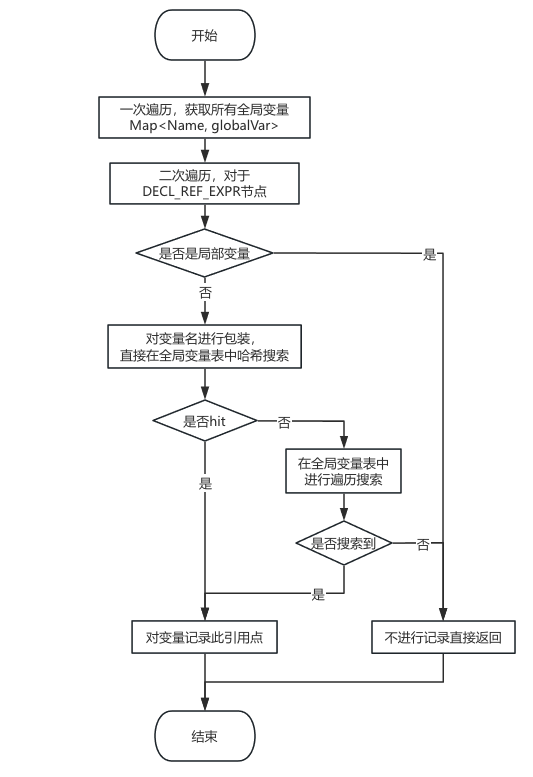
\includegraphics[width = 0.7\textwidth]{全局变量提取流程图.jpg}
\caption{全局变量提取流程图}
\end{figure}

第一次遍历获取所有的全局定义。首先提取所有的
VAR\_DECL 节点,它表示变量定义,然后提取节点中的变量名和变量类型。注
意,由于在 AST 中的节点标签中无法区分变量是否是全局的,所以这里根据节点在 AST
中的深度来判断是否是全局变量,并且在变量名前加上针对该项目文件的绝对路径,来
保证变量名的唯一性。在确定其为全局变量后,还需进一步提取该变量的作用域。在
C/C++语言中,static关键字可用于修饰变量和方法,意味着该变量或该方法只能在其所在文
件内使用,而不是全局可用,因此需要对其作用域进行判断。一次遍历提取到的结果是
一个全局变量表,这里使用哈希表 Map<Name, globalVar>的数据结构进行存储,方便对
全局变量进行查找。

第二次遍历的主要目的是提取全局变量的引用点。在方法节点子树中搜索
DECL\_REF\_EXPR 节点,该类型节点表示对变量的引用,这里首先判断被引用的变量是否是局部
变量,根据方法摘要表中该方法的相关信息可以判断,如果是则直接返回,因为我们不关心方法内的局部变量引用。如果不是,则证
明使用的是全局变量,首先在哈希表中进行查找该变量名,以节省检索时长,如果查找到了,说明
是在该文件中定义的全局变量,同时能够保证被 static 修饰的全局变
量的判断的准确性。如果没有查找到,则说明引用了别的文件中定义的全局方法,则在哈希
表中进行遍历查找,记录该全局变量被引用的方法。具体提取流程如图 2-3 所示。

分析结束后,将全局变量的信息进一步整理,组织为全局变量信息表,表的每一项表示一个全局变量的信息,每条信息由\textless \textit{globalVarID}, \textit{type}, \textit{use}, \textit{scope}, \textit{file}  \textgreater 共5部分组成,分别表示全局变量的唯一ID标识,变量类型,变量的引用点所在的方法,变量的作用域以及变量所在模块。



\section{基于依赖关系的变更影响分析}

在代码变更影响关系分析中,依赖关系传递闭包分析被广泛应用,这是一种基于静态依赖关系的技术手段,通过识别代码模块间的关联性划定受变更影响的范围\cite{2021Improving}。其核心思想是利用依赖关系的传递性,通过构建和分析依赖图,揭示所有可能受到影响的代码模块或单元。

\paragraph{构建依赖图}

以抽象语法树、全局变量信息表和方法摘要表为基础,构建程序的系统依赖图。图节点代表代码中的基本元素,本文中是方法和全局变量,而边则表示这些元素之间的依赖关系。依赖关系包括方法调用和全局变量变量引用,在全局变量信息表和方法摘要表中可直接提取依赖关系。生成边的原则如下:
\begin{itemize}
    \item 调用边(call):方法间的调用关系。如果方法A调用了方法B,在图中增加一条从节点A指向节点B的有向边。
    
    \item 引用边(use):方法和全局变量的引用关系。如果方法A引用的全局变量C,在图中增加一条从节点A指向节点C的有向边。
\end{itemize}

通过这种方式,依赖关系图不仅能够系统地表示代码中各个元素之间的直接依赖关系,还能为后续的变更影响分析提供结构化的图形模型。如图2-4为依赖图示例,该图中共有6个方法和3个全局变量,其静态依赖关系如图中的边所示。

\begin{figure}[h]
    \centering
    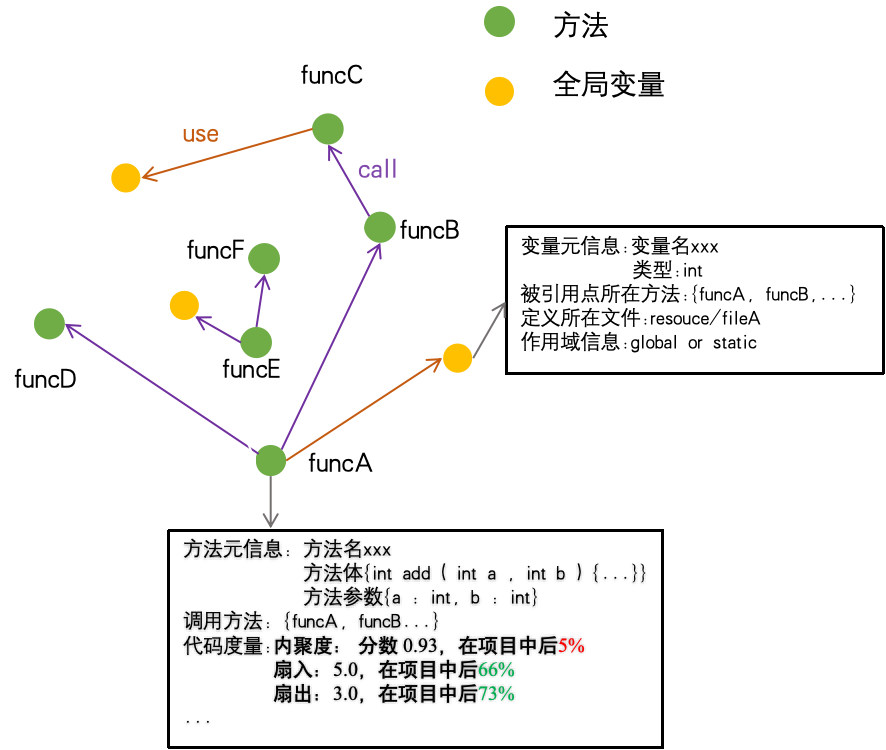
\includegraphics[width = 0.6\textwidth]{依赖关系示例.png}
    \caption{依赖图示例}
    \end{figure}

\paragraph{执行变更影响分析}

基于依赖图进行变更影响分析,这一过程旨在确定哪些方法在代码变更时可能受到影响,以及这些影响的传播路径。本文基于方法和方法之间的以下两种关系RBM(relationships between methods)对每一个方法识别当其变更时受影响的方法集IMS(impacted method set),定义如式(2-1)所示,以方法f和方法g的关系为例,CALL方法和RETURN分别代表f和g的调用和被调用关系。
\begin{equation}
\begin{array}{l}
R B M=C A L L \cup R E T U R N \text { where } \\
(f, g) \in C A L L \Longleftrightarrow f(\text { transitively)calls } g, \\
(f, g) \in R E T U R N \Longleftrightarrow f(\text { transitively)returns into } g
\end{array}
\end{equation}

对于依赖关系图中的每个节点,计算该节点的传递闭包。传递闭包是指从某个特定节点出发,根据上文定义的依赖关系和图的可达性,可以直接或间接到达的所有节点的集合,反映了节点之间的依赖链以及影响传播的范围。传递闭包的具体迭代模型如式2-2。

\begin{equation}
\begin{array}{l}
I M S^{(N)}=I M S_{C A L L}^{(N)} \cup I M S_{R E T U R N}^{(N)} \\
I M S_{ {RETURN }}^{(N+1)}=\bigcup_{{define } \in \left(I M S_{R E T U R N}^{(N)}}-I M S_{R E T U R N}^{(N-1)}\right)} I M S({ define }) \\
I M S_{C A L L}^{(N+1)}=\bigcup_{ {define } \in\left(I M S_{C A L L}^{(N)}\right)} I M S( { define }){, define } \in \\
\left(I M S_{C A L L}^{(N)}-I M S_{C A L L}^{(N-1)}\right) 
\end{array}
\end{equation}


其中N表示第N轮迭代,第N+1轮的迭代受N和N-1轮的影响,反映出软件系统中的变更的涟漪效应。为了高效地计算传递闭包,使用广度优先搜索遍历图中的各个节点及其依赖边,进而识别出所有直接或间接依赖于某个节点的其他节点。每次从某个节点出发时,都会跟踪并记录通过依赖关系可到达的所有节点,,最终得到的节点集合中,所有的节点都与初始变更的节点存在某种直接或间接的依赖关系。这些方法可以视为受变更影响的范围,意味着它们在该方法变更后,可能会因为依赖关系的传递而受到影响。通过这一分析,我们不仅可以识别出受影响的直接方法,还能揭示出那些通过多次间接依赖而受到影响的方法,帮助开发者全面了解变更的潜在影响范围。


在图 2-1 的例子中,方法 funcA 调用了 funcB 和funcD,funcB 调用了 funcC。在对 funcB 进行变更影响分析时,会直接影响到 funcA和funcC,根据依赖关系闭包,会间接影响到funcD。所以与 funcB 有变更影响关系的方法集合为\{funcA, funcC, funcD\} 。


\section{基于克隆关系的变更影响分析}
代码克隆(Code Clone)是指在代码中存在两段或多段内容相似或完全相同的代码片段。这些代码片段可能由于直接复制粘贴或手动修改而产生,通常是在软件开发过程中为了快速复用功能、减少重复实现或其他原因而引入的。代码克隆虽然可以在短期内提高开发效率,但在长期来看,可能对代码的维护和演化带来负面影响。

代码克隆主要分为以下三种类型:(1)完全克隆:两段代码完全相同,除了空白符、注释或格式化上的差异,这种克隆通常是直接复制粘贴的结果;(2)语法克隆:两段代码的结构和功能相同,但在变量名、方法名等命名上存在一些简单修改。(3) 修改克隆:两段代码基本相似,但在部分语句上有较大改动。例如,某些逻辑被修改、删除或添加。这种克隆通常反映了代码的部分复用。

在项目代码中,克隆的代码片段是完全或部分相同的,因此它们在逻辑上往往具有相同的功能或行为。如果对其中一个克隆片段进行了变更(例如修复了一个 bug、添加功能或进行优化),那么在其他地方相同或相似的代码也可能需要同步修改,否则可能会导致系统的不一致性或错误,这是典型的逻辑型变更影响关系。

因此,本文基于方法间的克隆关系进行变更影响分析。追踪在代码变更过程中,克隆代码之间的相互依赖及其潜在影响,从而为开发者的安全变更提供参考。这一方法不仅有助于揭示代码重复带来的潜在风险,还能为开发人员提供系统的变更影响评估,从而优化代码维护和改进的决策过程,推动软件质量的持续提升。

该方法主要分为两步,首先对源程序进行预处理,通过代码分段及代码指纹提取的方式对源程序进行编码,生成代码序列数据库。随后利用频繁模式挖掘算法ClaSP得到克隆代码列表,具体的算法流程如图3-2所示。

\begin{figure}[h]
\centering
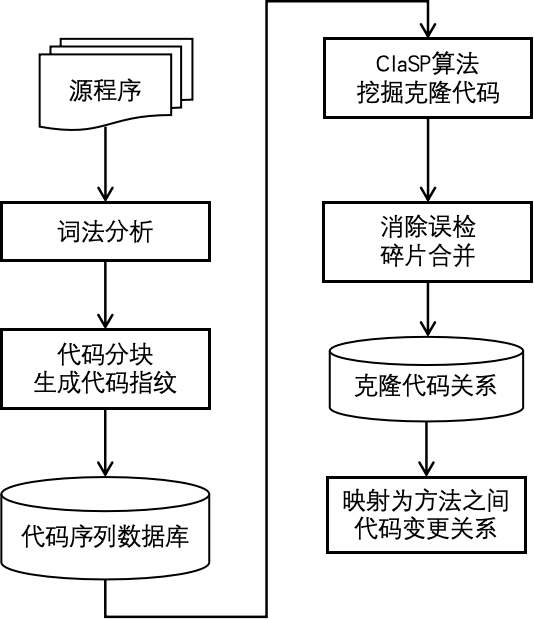
\includegraphics[width = 0.4\textwidth]{代码克隆流程}
\caption{基于代码克隆的变更影响分析方法流程}
\end{figure}



\subsection{代码预处理和分块}

为了精确有效地检测代码克隆,需先对源代码进行详细的预处理,以消除可能影响克隆检测准确性的各种干扰因素。

\paragraph{代码预处理}

\begin{itemize}
    \item 去除注释:注释通常用于解释代码的意图,并不直接影响程序的执行,但不同的代码实现中注释内容可能存在差异,这会导致本质相同的代码片段由于注释的不同而被误判为非克隆。因此,去除注释可以避免注释的差异干扰克隆检测的结果,从而确保算法专注于代码的实际逻辑。
    
    \item 去除头文件引用语句:在C/C++程序中,源代码文件往往会包含多个头文件,而不同的源文件可能引用相同的头文件。如果不对头文件进行统一的处理,算法就可能在不同的源文件中检测头文件引用的代码克隆情况,进而导致无谓的计算冗余。这不仅增加了处理的时间和空间复杂度,还可能影响克隆检测的效率和准确性。
    
    \item 程序标准化:为了避免因变量名的变化导致漏检,在方法内部对变量名进行统一标准化处理,将所有局部变量和参数名替换为预定义的标准变量名,从而消除变量名不同带来的影响。这一过程有助于聚焦于代码的逻辑和功能层面,而非单纯依赖变量命名的差异,从而提高克隆检测的准确性和可靠性。

\end{itemize}

通过上述预处理过程,可以生成一个清晰、标准化的源代码文件,不仅消除了无关的噪声,还确保了源代码的逻辑和结构能够被准确捕捉,为后续的克隆检测提供了高质量的输入数据。


\paragraph{代码分块}

代码分块的主要目的是将代码拆解成更小、更易于对比的单元,从而提高克隆检测的准确性。本文的代码分块策略按代码结构的不同分为几类,

\begin{itemize}
    \item 顺序结构:按固定行数分块,行数可由用户定义,默认为6行一块。行数越小则识别结果越精准,越能识别更细小的代码克隆情况。
    
    \item 控制结构:将选择结构(if、then、else、endif、switch)、循环结构(while、for)、和域结构(\{、\})共同描述为控制结构识别并根据关键分块词进行分块。这是由于控制语句是代码逻辑的重要分界点,将它们作为分块的标准可以确保检测系统能聚焦于实际功能的逻辑边界。
\end{itemize}


此外,在代码克隆检测中,还需要遵循一些附加规则以确保检测的准确性和一致性。
\begin{itemize}
    \item 大括号不被视为代码块的一部分:不同的开发者在代码排版上可能存在差异,例如有的开发者将大括号置于同行,而另一些则习惯将大括号另起一行。为了避免这种格式差异对克隆检测结果产生干扰,大括号被排除在代码块之外,从而确保检测过程更侧重于代码的逻辑结构,而非视觉格式上的不同。
    
    \item 分块过程中记录位置信息:包括代码块所在的文件路径、代码块的起始行号和终止行号、代码块的总行数,以及每个块包含的具体行数共5个信息。通过这种方式,不仅能够清晰地标识出每个代码块的位置,还能为后续的克隆碎片合并提供必要的上下文支持。
\end{itemize}

通过这些步骤和规则,代码被拆分成更小、更一致的单元,使克隆检测能够更加高效且精准地识别功能相似的代码块。


\paragraph{代码指纹提取}

这一步遍历代码块的每一行语句,将每行语句转化为数字序列,再将所有数字序列合并,转化为代码块的“指纹”。该指纹将代表代码片段用于识别代码片段之间的相似性或重复性。通过这种方式,不同的代码片段信息被压缩,转换为具有独特标识符的形式,从而在后续的分析中实现高效的比较和匹配。鉴于哈希算法在计算上的高效性与实现的简便性,它在生成代码指纹方面具有显著的优势。因此,本文选择采用冲突率较低的hashpjw算法提取代码指纹,以确保在保证高效性的同时,能够快速、准确地对代码进行相似性分析和重复性检测。


\subsection{基于代码克隆检测的变更影响关系提取}
序列数据挖掘(Sequence Data Mining,SDM)是时序数据挖掘领域的一个重要研究方向,旨在从给定的输入数据库中,探索在大量对象之间随时间频繁出现的模式。判断一个模式是否具有意义的阈值被称为最小支持度。SDM 已被广泛研究,并在多个领域得到了应用,如 DNA 序列中的基序发现、顾客购买序列分析、网页点击流分析等。本文中,将代码指纹片段作为序列,利用序列数据挖掘算法,挖掘频繁出现的模式,提取对应的代码克隆序列。

(1)数据挖掘领域基本概念

项集\cite{2013ClaSP}:设有一个集合 \( I = \{i_1, i_2, \dots, i_n\} \),其中 \( i_i \) 表示一个项。项集即为这个项的非空子集。一个项可以出现在多个项集中,但同一项集中的每个项只能出现一次,即不允许项集包含重复的项。在本文中,项集指的是代码行的指纹。

序列\cite{2013ClaSP}:序列是一个由项集组成的有序列表,记作 \( s = (s_1, s_2, \dots, s_n) \),其中每个 \( s_i \) 是项集。每个项集 \( s_i \) 可以进一步表示为 \( (x_1, x_2, \dots, x_m) \),其中 \( x_m \) 是项。本文中序列指代码块的指纹。

子序列\cite{2013ClaSP}:考虑两个序列 \( \alpha = (a_1, a_2, \dots, a_n) \) 和 \( \beta = (b_1, b_2, \dots, b_m) \),如果存在一组整数 \( 1 \leq j_1 < j_2 < \dots < j_n \leq m \),使得序列 \( (a_{j_1}, a_{j_2}, \dots, a_{j_n}) \) 是序列 \( \beta \) 的子序列,则称序列 \( \alpha \) 为序列 \( \beta \) 的子序列,序列 \( \beta \) 为序列 \( \alpha \) 的超序列。

序列数据库\cite{2013ClaSP}:序列数据库是由一组元组 \( \langle \text{sid}, s \rangle \) 构成的集合,其中 \( \text{sid} \) 为序列的标识符,\( s \) 为序列。如果序列 \( \alpha \) 是元组 \( \langle \text{sid}, s \rangle \) 中序列 \( s \) 的子序列,则称该元组包含序列 \( \alpha \)。序列数据库中包含序列 \( \alpha \) 的元组的数量被称为序列 \( \alpha \) 的支持度。本文中指的是项目代码所有分块的集合。

频繁子序列\cite{2013ClaSP}:给定一个正整数 \( \text{min\_support} \) 作为支持度阈值,如果序列 \( \alpha \) 的支持度大于或等于 \( \text{min\_support} \),则称序列 \( \alpha \) 为频繁子序列。所有频繁子序列的集合记为 \( FS \),即Frequent Subsequenc。


序列支持度:记作 \( \sigma(\alpha, D) \),是指在数据库 \( D \) 中包含序列 \( \alpha \) 的序列的总数。如果一个模式或序列至少出现给定的用户指定阈值 \( \text{min\_support} \),即最小支持度,则称其为频繁序列。频繁序列挖掘的问题就是在给定的输入数据库中,找到满足最小支持度阈值的频繁序列集合 \( FS \)。本文中即是找到频繁出现的代码。


闭合序列:如果一个频繁序列 \( \alpha \) 没有其他超序列与其具有相同的支持度,则称 \( \alpha \) 为闭合序列。所有频繁闭合序列的集合记作 \( FCS \)。更正式地说,若对所有 \( \beta \in FS \),有 \( \alpha \subseteq \beta \) 且 \( \sigma(\alpha, D) = \sigma(\beta, D) \),则 \( \alpha \in FCS \)。

闭合序列挖掘的问题就是在给定的输入数据库中,找到满足最小支持度阈值的闭合序列集合 \( FCS \)。显然,频繁闭合序列的集合要小于所有频繁序列的集合。这是因为在频繁模式的集合中,很多模式可能是冗余的。例如,某些频繁模式的支持度相同,且其中一个是另一个的超序列。对于这些模式而言,冗余的超序列模式没有提供比其子序列模式更多的信息。闭合频繁模式的引入可以去除这些冗余,保留那些最具代表性和信息量的模式。

这里举例说明,表3-1为序列数据库示例,这里设定最小支持度阈值为2。

\begin{table}[htbp]
\caption{序列数据库示例}
\vspace{0.5em}\centering\wuhao
\begin{tabular}{cccc}
\toprule
序列id(sid) & 序列 \\
\midrule
1 &  \langle (a)(ab)(bc)\rangle\\
2 & \langle (a)(abc) \rangle\\
3 & \langle (d)(a)(ab)(bc) \rangle\\
4 & \langle  (d)(ad)\rangle\\
\bottomrule
\end{tabular}
\end{table}

在这个例子中,第一个序列中有3个项集,分别是(a),(ab)和(bc),以此类推。根据上述概念计算得到,这个例子中的闭合频繁序列FCS=\(\{ \langle (a)\rangle, \langle (d)(a)\rangle, \langle (a)(ab)\rangle, \langle (a)(bc)\rangle, \langle (a)(ab)(bc)\rangle \}\), 共5个,而频繁序列有27个。因此识别闭合频繁模式具有重要的压缩性,并且模式信息也是不丢失的。

(2)ClaSP算法

ClaSP算法主要分为两步,首先生成频繁序列,作为频繁闭合序列的候选FCC(Frequent Closed Candidates)。第二步执行剪枝,从候选中剔除所有非闭合的序列,最终得到精确的FCS。主要的算法流程如3-1所示。

\begin{algorithm}
\caption{ClaSP算法}
\begin{algorithmic}
\KwIn{序列数据库}
\KwOut{频繁闭合序列集 $FCS$}
\State $F_1 \gets \{\text{频繁 1-序列}\}$ \\
\State $FCC \gets \emptyset$, $FCS \gets \emptyset$  \\
\For{\textnormal{all} $i \in F_1$} {
    \State $F_{ie} \gets \{\text{频繁 1-序列的长大于i的扩展序列 } \}$ \\
    \State $FCC_i \gets \text{DFS-Pruning}(i, F_1, F_{ie})$ \\
    \State $FCC \gets FCC \cup FCC_i$\\}
\EndFor
\State $FCS \gets \text{N-ClosedStep}(FCC)$
\end{algorithmic}
\end{algorithm}


首先找到所有的频繁的1-序列(即长度为1的序列),然后,对于所有频繁的1序列,递归地调用DFS-Pruning方法来探索相应的子树(通过进行深度优先搜索)。对所有频率为1的序列进行此处理,得到FCC,最后,算法结束去除FCC中出现的非闭合序列。


\begin{algorithm}[htbp]
\caption{DFS-Pruning算法}
\KwIn{当前模式 $p$, 候选项集 $S_n$ 和 $I_n$}
\KwOut{更新后的频繁模式集 $FCC$}

$Stemp \gets \emptyset$ 
$Itemp \gets \emptyset$ 
$F_i \gets \emptyset$ 
$P_s \gets \emptyset$ 
$P_i \gets \emptyset$ \\
\If{$\neg \text{checkAvoidable}(p, I(D_p))$}{
    \For{all $i \in S_n$}{
        \If{$p' = (s_1, s_2, \dots, s_n, \{i\})$ is frequent}{
            $Stemp \gets Stemp \cup \{i\}$ \\
            $P_s \gets P_s \cup \{p'\}$ \\
        }
    }
    $F_i \gets F_i \cup P_s \cup \text{ExpSiblings}(P_s, Stemp, Stemp)$ \\
    \For{all $i \in I_n$}{
        \If{$p' = (s_1, s_2, \dots, s_n \cup \{i\})$ is frequent}{
            $Itemp \gets Itemp \cup \{i\}$ \\
            $P_i \gets P_i \cup \{p'\}$ \\
        }
    }
    $F_i \gets F_i \cup P_i \cup \text{ExpSiblings}(P_s, Stemp, Itemp)$ \\
}
\Return{$F_i$} \\
\end{algorithm}
    

其中DFS-Pruning 算法的核心流程如3-2所示。通过递归生成候选模式(包括 s-扩展和 i-扩展,分别在模式末尾和任意位置添加新元素)并检查其支持度,最终返回以当前模式 $p$ 为前缀的所有频繁模式集。算法输入包括当前频繁模式 $p$ 以及用于执行扩展操作的候选项集 $S_n$ 和 $I_n$。

在 s-扩展阶段,算法遍历 $S_n$ 中的每个候选项 $i$,检查扩展后的模式是否为频繁模式。若为频繁模式,则将其加入 $Stemp$ 和 $P_s$ 中,并通过递归调用 ExpSiblings 方法继续扩展。i-扩展部分则类似,遍历 $I_n$ 中的候选项,检查并加入频繁扩展模式到 $Itemp$ 和 $P_i$ 中,最终进行 i-扩展的剪枝处理。

最终,算法返回以模式 $p$ 为前缀的所有频繁模式集 $F_i$,其中包括通过 s-扩展和 i-扩展生成的所有频繁模式。这些操作通过递归遍历模式树,确保高效地发现所有频繁模式。


剪枝时,通过检查对应模式的子序列和超序列的支持度,将序列的节点进行合并,防止继续遍历冗余节点。最终得到的FCS即为所有克隆代码集。

(3)合并碎片

由于先前的代码分段处理导致克隆代码呈现为片段间的克隆关系,为了恢复代码的完整性,进一步对这些碎片进行合并。基于每段代码的位置信息,将属于同一方法的碎片进行合理整合,从而重建方法间的克隆关系。通过这种方式,最终得到的是方法与方法之间的克隆关系,反映了不同方法之间的相似性。

这种方法间的克隆关系不仅揭示了代码的重复性,还反映了不同方法之间在代码修改过程中的潜在影响。方法与方法之间的克隆关系可以被视为一种变更传播的路径,指示了某一方法的修改可能如何影响其他方法。因此,提取出的克隆关系即代表了方法之间的变更影响关系。

\section{基于变更历史和共现关联关系的变更影响分析}
\subsection{代码变更历史提取}

在软件工程中,分析代码变更历史是理解软件演化重要手段之一。在开发者对项目进行维护的过程中,通常是以一个提交(commit)为单位进行功能上的变更。当进入新的维护工作时,如对同一功能进行升级等,通常的做法是参考前人的开发历史,对当前开发工作做指导,以防止变更的不完全。基于这一特点,本文设计了基于变更历史和共现关联关系的变更影响分析方法,分析对象是软件项目的变更历史。该方法能够提取蕴含在代码变更历史中的变更影响关系,尤其适用于具有丰富变更记录的软件项目。

该方法的核心原理是:在代码变更历史中,频繁同时更改的代码片段,通常存在着某种潜在的变更影响关系。这种变更影响关系不仅仅局限于静态结构上的依赖,还包括功能上的耦合和实现上的相互作用。因此,通过对这些历史变更数据的深入挖掘和分析,我们可以揭示出更丰富的逻辑型变更关系。

本方法的具体过程主要分为两部分,首先是对代码变更历史的收集与整理,然后通过数据挖掘技术提取并分析方法之间的变更影响关系。其中代码变更历史提取具体流程如下:

(1)收集项目代码库及变更历史记录

由于 Git 是现代软件开发中最广泛使用的版本控制工具,因此,本文的分析主要集中在 Git 项目上。首先,克隆项目的代码库到本地,项目中的.git文件夹中包含了版本变更历史记录,包括所有提交(commit)记录等。每个提交代表着代码库的一次变更,包含了代码的修改、删除或新增文件等信息。通过git log命令获取每次commit的详细信息,包括每个提交的哈希值、作者、日期和提交信息等。

(2)提取每个提交的变更信息

每个提交不仅仅是一个单一的代码变更,往往涉及多个文件的更改。因此,对于每个提交,运行git show <commitHash>命令,查看该提交引入的代码变更(即“diff”或差异),这会显示哪些文件被修改、添加或删除,本文主要关注标记为“修改”的文件,这些修改的文件中包含了具体的代码变化,即代码行的增、删、改操作,记录该commit引起的所有发生变更的代码行。

(3)定位变更代码行所属的方法

在提取了具体的代码变化后,定位这些变化的代码行所在的方法。通过libclang分析变化前文件得到的抽象语法树可获取每个方法对应的代码行,将变更的代码行的位置与方法位置进行匹配,进而得到变更的代码行所在的方法。

(4)提取变更方法与提交的关系

对于每个提交,提取出所有受影响的方法(即发生变化的方法),并将这些方法构成一个变更方法列表。这个列表反映了在特定提交中发生变更的所有方法,并为后续的变更影响分析提供了基础数据。用Map<commitID, List<Methods>>的结构存储每个commit变更的方法,作为序列数据库,便于后续分析与处理。


\subsection{基于共现关联挖掘的变更影响关系提取}

基于关联规则(Association Rules)的数据挖掘方法是反映事物之间相互依存性和关联性的一个重要数据挖掘技术,旨在从大量数据中挖掘出有价值的项之间的相关关系。共现关系可以视为关联规则的一种表现形式,它描述了在给定集合中,某一组项(或特征)经常出现在同一事务中。例如,在零售分析中,常见的共现关系是“购买了面包的顾客通常也会购买牛奶”。在这种情况下,“面包”和“牛奶”是一对共现项。

在本文的代码变更影响分析中,共现关系描述的是在一次提交中,哪些方法经常同时发生变更。如果两个方法在多个提交中频繁一起变动,则它们之间可能存在某种依赖关系或变更影响关系。通过分析这些方法在多个提交中被频繁同时修改的情况,我们能够识别方法之间的变更影响路径,从而揭示它们的潜在关联性。


常用的频繁项集的评估标准有支持度和置信度。支持度表示共现项在数据集中出现的次数占总数据集的比重,用于衡量一组项在数据集中的普遍程度。在代码变更分析中,支持度表示某一方法对在多个提交中同时出现的频率,计算公式如3-3.

\begin{equation}
Support(funcA,funcB)=\frac{num(AB\text{共现})}{num(AllCommits)}
\end{equation}

置信度表示共现项中一个出现后,另一个项出现的概率。变更分析中,置信度度量表示当方法A被修改时,方法B被修改的概率,计算公式如3-4。

\begin{equation}
Confidence(funcA\Leftarrow funcB)=\frac{P(AB\text{共现})}{P(B\text{出现})}
\end{equation}

在前文提取的序列数据库中,进行如下步骤的计算,详细流程见算法3-3。

首先,遍历序列数据库,搜索并得到候选 1 项集,即包含单个元素的项集,这些元素代表在变更历史中被修改过的方法。计算对应的支持度,剪枝去掉低于支持度的1项集,得到频繁1项集,频繁 1 项集中的元素反映了在变更历史中频繁出现的被修改方法。

基于频繁 1 项集中的元素,通过连接操作生成候选的频繁 2 项集。通过再次遍历序列数据库,计算候选频繁 2 项集的支持度,并筛选去除那些支持度低于设定阈值的项集。经过这一筛选步骤后,得到真正的频繁 2 项集。频繁 2 项集中的元素表示了那些在变更历史中频繁同时被修改的两个方法对。

在得到频繁 2 项集之后,进一步筛选出置信度高于或等于设定阈值的方法对。最终,留下的即为那些频繁同时变更,并且存在强关联关系的的方法对,表明它们在变更过程中有着较为显著的相互依赖关系,即方法对之间的变更影响关系。

\begin{algorithm}
\caption{变更影响方法对挖掘算法}
\begin{algorithmic}
\KwIn{序列数据库 $D$, 支持度阈值 $min\_sup$, 置信度阈值 $min\_conf$}
\KwOut{变更影响方法对 $change\_impact\_pairs$}
\State $F_1 \gets \emptyset$  \# 频繁1项集\\  
\For{all $f \in D$} {
    \If{support$(f) \geq min\_sup$} {
        $F_1 \gets F_1 \cup f$
    }
} \\
\State $F_2 \gets \emptyset$  \# 频繁2项集\\ 
\For{all $(f_1, f_2) \in P = \{ (f_i, f_j) \mid f_i, f_j \in F_1, i \neq j \}$} {
    \If{$\text{Support}(f_1, f_2) \geq min\_sup$} {
        $F_2 \gets F_2 \cup (f_1, f_2)$
    }
}

\State $change\_impact\_pairs \gets \emptyset$ \\ 
\For{all  $(f_1, f_2) \in F_2$} {
    \If{confidence$(f_1, f_2) \geq min\_conf$} {
        $change\_impact\_pairs \gets change\_impact\_pairs \cup (f_1, f_2)$
    }
}
\Return{$change\_impact\_pairs$}
\end{algorithmic}
\end{algorithm}

\section{基于深度学习的变更影响分析}

\subsection{数据集来源和数据清洗}

当项目代码拥有丰富的变更历史时,可以通过前文中介绍的数据挖掘方法,提取具有变更影响关系的方法对。这种方法通过分析历史提交记录中方法间的共现频率,识别出在多次变更中相互依赖或相互影响的方法。然而,并不是所有软件项目都有变更历史可供我们分析,在仅有项目源代码的情况下,数据挖掘方法无法直接应用,但是只使用基于依赖闭包和基于克隆代码的方法,则无法识别除这两种关系外更深层次的变更影响。因此本文提出基于深度学习的变更影响分析方法,通过训练深度学习模型,对变更影响关系进行预测,以弥补另两种分析方法的不足。

为了识别那些来源除了依赖关系和代码克隆得到的代码变更影响关系,需要收集包含深层变更影响关系的方法对。而3.4节中根据数据挖掘的变更影响关系分析的方法,恰巧具有这一特征。该方法可以识别出那些在多个提交记录中频繁同时发生变更的方法对,由于我们的标准设置十分严格,因此识别的变更影响关系具有较强的可靠性,可作为数据集的正例进行收集。此外,为了构建平衡的数据集,通过对项目中的方法进行随机抽样,从中选取一些不具有变更影响关系的方法对,作为数据集的负例进行收集。

在数据集收集过程中,本文面临了几个挑战。首先,一些看似活跃的项目(例如频繁提交的项目)实际上并未挖掘到大量可用数据。分析原因是由于项目规模较大,文件数量庞大,开发者的工作内容往往不具有交集,大部分的方法不会被二次更改,因此难以出现频繁的样例。其次,对于一些发展时间较长的项目,因为提交记录众多(如数万次提交),所以在收集数据时需要处理大量的提交,这使得数据处理的过程非常耗时。

为了解决这些问题,本文在选择项目时设定了一些标准。首先,优先选择规模适中的项目,这些项目既足够活跃,又不会因为过于庞大的代码库而导致数据处理困难。同时,考虑到提交记录较多的项目可能导致数据量过大,本文限制了采集范围,只选择了最近的提交记录(例如最新的2000个提交)。这一策略有两个主要考虑:一方面,确保数据量足够大,以支持后续的挖掘工作;另一方面,聚焦于那些近期频繁变动的方法,排除较为稳定且变化较少的旧函数,从而更好地反映出当前项目的活跃度和变更趋势。

\subsection{基于代码预训练模型的变更影响关系预测}

基于深度学习的影响关系预测任务的输入为两个方法体,输出为两个方法之间存在变更影响关系的概率,概率越接近 1,表明这两个方法之间有关系的可能性越大。

考虑到代码理解的复杂性与深度,本文采用了基于预训练模型的代码表示学习方法,选择了 CodeBERT 作为核心模型。CodeBERT 是一种专为程序代码设计的预训练语言模型,通过大规模的代码语料库预训练,能够学习到代码中的丰富语法结构和语义信息。经过 CodeBERT 模型的表示学习,所得到的向量不仅包含了每个方法体的语法特征,还能够编码代码中的语义关系及其他潜在的编程特征。模型架构如图3-3所示。

\begin{figure}[h]
\centering
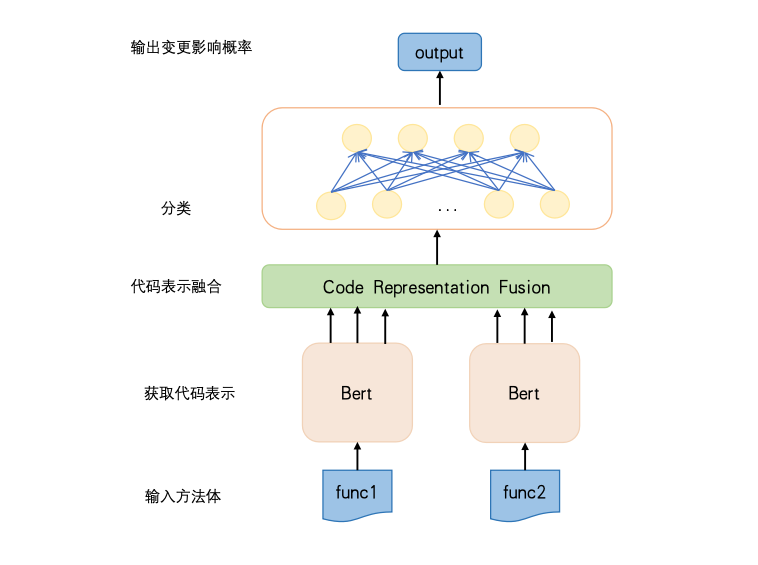
\includegraphics[width = 0.8\textwidth]{模型架构3.jpg}
\caption{基于代码预训练的深度学习模型架构}
\end{figure}


首先,将两个方法体$ F_a, F_b$,先通过代码预训练模型进行编码

\begin{align}
H_a=&Encoder(F_a) \in \mathbb{R}^{(len,dim)} \\
E_a=&mean(H_a[1:...]) \in \mathbb{R}^{(dim)}
\end{align}

得到方法的向量化表示$ E_a, E_b$,通过拼接融合这两个向量,将融合后的向量表示送入一个由两层组成的多层感知机(Multilayer Perceptron,MLP)中,再通过 softmax 层进行分类处理,将模型的输出转化为一个概率分布,表示两个方法体之间存在关系的概率。

\begin{align}
E_{a,b}=Concat(E_a,E_b)& \in \mathbb{R}^{(dim*2)} \\
logits_{a,b}=MLP(E_{a,b})&=FFN(ReLU(FFN(E_{a,b}))) \\
FFN(x)&=Wx+b\\
ReLu(x)&=max(0,x)\\
logits_{a,b}& \in \mathbb{R}^{(2)}
\end{align}

最后与真实标签计算交叉熵损失,得到loss,计算梯度,优化模型参数
\begin{align}
loss=CrossEntryLoss(logits_{a,b}, Label)
\end{align}


\section{实验结果与分析}

\subsection{实验数据与评价方式}

\paragraph{实验数据}

本文从影响力或社区活跃程度的角度出发,收集了表2-2中所示的软件项目为被测项目进行实验。这些项目在github上的收藏数均在千以上,说明这些项目在开源社区中有着一定的影响力,使用范围比较广泛。除antiword项目之外,其他项目有着比较活跃的社区,说明其还在不断更新迭代过程中,所以能提供较为丰富的变更历史,以供数据挖掘方法的实验分析。

\begin{table}[htbp]
\caption{被测项目}
\vspace{0.5em}\centering\wuhao
\begin{tabular}{cp{6cm}ccc}
\toprule
项目名称 & 项目简介 & 代码行数& 提交数 & 收藏数 \\
\midrule
TheAlgorithms & 各种算法的开源实现,涵盖了计算机科学、数学和统计学等领域 & 24645 & 1536 & 57k \\
antiword-0.37 & 提取 Microsoft Word 文档内容的工具 & 34725& - & 13k\\
jemalloc-5.3.0 & 通用的malloc(3)实现,强调碎片避免和可扩展的并发支
持  &83525& 3530 & 9k \\
libbpf-1.1 & linux 内核观测技术的一个脚手架库 & 127927 & 2375 & 1.9k \\
librdkafka-2.1.0& Apache Kafka 的 C/C++ 客户端库 & 154951 & 4430 & 18k \\
FFmpegKit-5.1.0 & FFmpeg 工具包 & 450998 & 369 & 3.7k \\

\bottomrule
\end{tabular}
\end{table}


根据每个示例项目的上一个版本和示例版本间的版本变更,分别各自选取50个变更方法,通过分析commit得到真实的被影响方法集AIS(Actual Impact Set),作为测试集,这里分别统计了依赖型和逻辑型的变更影响关系,得到的数据如表2-3所示。再分别通过前述方法进行检测,得到估计的被影响方法集EIS(Estimated Impact Set),通过评价指标评估方法的有效性。

\begin{table}[htbp]
\caption{被测项目数据统计}
\vspace{0.5em}\centering\wuhao
\begin{tabular}{cccccc}
\toprule
项目名称 & commit数 & 变更点数 & 依赖型AIS & 逻辑型AIS & 总计 \\
\midrule
TheAlgorithms &  & 50 & 162 & 34 & 196\\
antiword-0.37 & - & 50 & 197 & 89 & 186 \\
jemalloc-5.3.0 &   & 50 & 112 & 21 & 133 \\
libbpf-1.1 &  & 50 & 322 & 27 & 349 \\
librdkafka-2.1.0 &  & 50 & 153 & 43 & 203\\
FFmpegKit-5.1.0 &  & 50 & 175 & 27 & 202\\
总计 &  & 300 & 1121 & 241 & 1362 \\
\bottomrule
\end{tabular}
\end{table}


基于深度学习的变更影响分析方法的数据集收集方式如3.5.1节所述,为了保证测试集和训练集的不重叠性,在经过挖掘和清洗后得到的关系中排除上述测试变更点。得到的数据集统计信息如表3-2所示,共7351对数据,按照训练、验证、测试集 为 6:2:2 进行训练和测试。这里排除了antiword项目,因为该项目并没有官方维护的github仓库,因此无法获得足够的历史变更。

\begin{table}[htbp]
\caption{数据集统计信息}
\vspace{0.5em}\centering\wuhao
\begin{tabular}{cccc}
\toprule
项目名称 & 正例对数 & 负例对数 & 总对数 \\
\midrule
TheAlgorithms & 97 & 1000 & 1097 \\
jemalloc-5.3.0 & 593 & 1000 & 1593 \\
libbpf-1.1 & 401 & 1000 & 1401 \\
librdkafka-2.1.0 & 932  & 1000 & 1932 \\
FFmpegKit-5.1.0 & 17 & 1000 & 1017 \\ 
总计 & 2040 & 5000 & 7040 \\
\bottomrule
\end{tabular}
\end{table}

\paragraph{评价指标}

评价指标如式(3-13)(3-14)(3-15)所示,真实的被影响方法表示为AIS(Actual Impact Set),每种方法检测得到的结果为估计的被影响方法EIS(Estimated Impact Set),按逻辑型和依赖型对关系进行划分,根据这两个值计算精确度、召回率和F-measure,这三种评价指标在信息检索的场景下被广泛使用,本章中用于评价变更影响分析方法的有效性。
\begin{equation}
{precision} = \frac{|EIS \cap AIS|}{|EIS|}
\end{equation}

\begin{equation}
{recall} = \frac{|EIS \cap AIS|}{|AIS|}
\end{equation}

\begin{equation}
F-measure = \frac{2 \times precision \times recall}{precision + recall}
\end{equation}

\subsection{实验设置与评价方式}
1. 实验设置

(1)深度学习实验设置

针对基于深度学习的变更影响分析方法。本文使用了CodeBERTa-small-v1和codebert-base-mlm两个模型分别作为代码表示学习模型,得到的代码表示为768维,融合时使用的MLP的每层维数为(768*2,64,2)。

模型的参数设置如表3-3。

\begin{table}[htbp]
\caption{模型参数设置}
\vspace{0.5em}\centering\wuhao
\begin{tabular}{cccc}
\toprule
超参数 & 数值  \\
\midrule
Token embedding size & 768 \\
codeBERT learning-rate  & 1e-5 \\
codeBERT dropout & 0.4 \\
Classifier learning-rate& 1e-4 \\ 
Adam \beta_1  & 0.95  \\
Adam \beta_2 & 0.999  \\
batch\_size & 64 \\
\bottomrule
\end{tabular}
\end{table}    

\subsection{实验结果与分析}

基于深度学习的方法在数据集上的实验结果如表3-5所示,从总体上来看,两个模型的性能均表现出色,深入分析可以发现两个模型各有所长。

\begin{table}[htbp]
\caption{基于代码预训练模型的变更影响关系预测实验结果}
\vspace{0.5em}\centering\wuhao
\begin{tabular}{cccc}
\toprule
模型& F-measure & recall & precision \\
\midrule
CodeBERTa-small-v1 & 91.8 & 86.1 & 98.2 \\
codebert-base-mlm  & 87.1 & 100.0  & 77.1 \\
\bottomrule
\end{tabular}
\end{table}

CodeBERTa-small-v1 模型更强调预测出的正例的真实性和准确性。这意味着它在确保预测结果的准确性方面做得很好,但可能会导致一些正确的情况被漏掉,即存在漏报。此外由于"small"模型的规模较小,参数数量较少,这可能会使得模型在训练过程中更容易发生过拟合现象。而CodeBERT-base-mlm 模型则更注重捕捉尽可能多的正样本。这个模型虽然能够覆盖更多的正例,但也引入了更多误报。但是该模型参数更多,具备更强的泛化能力,通常能够更好地适应新的数据集。

深度学习方法在实际应用中的效果如图3-5中所示,其可以挖掘两种类型的变更影响关系。与数据挖掘方法相比,该方法更倾向于挖掘逻辑型变更影响关系,表现为逻辑型报告比例相较于数据挖掘方法更多,这或许是由于数据集的不平衡所导致的。尽管两种类型的准确率均不高,但仍能从检测出的样例中发现一定的实际应用价值,在没有代码变更历史的软件项目中,可以作为对传统方法的补充。



\paragraph{实验设置}


本文将基于变更历史和共现关联关系方法的挖掘算法置信度设置为1。具体而言,对于方法A,记录其在所有提交记录中出现的次数为\(N_A\),并统计在这些提交中,其他方法B出现的次数为\(N_B\)。如果在所有提交中,方法A出现时,方法B的出现频率达到\(N_A \backslash N_B = 1\)
则认为方法对 $(A, B)$ 存在变更影响关系。换句话说,置信度为1表示每当方法A被修改时,方法B也必然随之修改,从而确认这两个方法的变更是紧密关联的,并且它们的修改行为是同步的。

本文将基于变更历史和共现关联关系方法的支持度设为2进行实验,与其他方法进行对比。意味着方法A和方法B在多个提交中同时出现的次数必须至少为2次,才能认为这两个方法之间可能存在变更影响关系。支持度的设定要求方法对 $(A, B)$ 在变更历史中有一定的共现频率,从而能够确保所识别的变更影响关系具有一定的统计显著性,避免偶然性因素的干扰。

本文进一步将支持度设置为2和3进行方法内的对比实验,通过对比实验结果,研究支持度的不同对于方法性能的影响。

\subsection{实验结果与对比分析}

本节将通过实验对比来评估本章中提出的基于深度学习的变更影响分析方法的性能,这里主要讨论下列三个问题:

RQ1:本章提出的基于深度学习的方法能否有效检测变更影响关系?与其他方法相比,它在精确率,召回率和F-measure上表现如何?

RQ2:四种方法在提取依赖型(DB)和逻辑型(LB)的变更影响关系上各自的优势如何?尤其是对于逻辑型的影响关系是否具有实际意义?分别适用于哪些特殊场景?又各自有怎样的局限性?


\textbf{1.针对于RQ1的实验}

三种方法的实验结果如表3-4所示。


整体上讲,基于共现关系的方法表现最好,其F-measure在所有方法中表现最优。这表明,代码变更历史中方法的共现关系的确蕴含了大量能够有效揭示变更影响关系的信息。这是因为变更历史中都是前人对软件项目进行变更的记录,这样的提交由开发者精确变更,并经历过开源项目中非常严格的审查过程才合入主分支,因此较为准确地反映了代码变更中的实际操作,从而也能将过去的开发模式反映在数据挖掘的结果集中。

\begin{table}[htbp]
\caption{变更影响实验结果 - F-measure/召回率/精确度}
\vspace{0.5em}\centering\wuhao
\begin{tabular}{cccccccc}
\toprule
方法 & F-measure & recall & precision  \\
\midrule
依赖关系 & 42.2 & 81.3 & 28.5  \\
克隆关系 & 6.4 & 3.3 &  92.0 \\
共现关系 & 74.8 & 68.7 & 82.0 \\
\bottomrule
\end{tabular}
\end{table}

而另外两种方法表现则较为失衡。基于依赖关系闭包的方法表现为召回率较高而准确率很低,仅为28.5\%。这是由于依赖闭包方法本身的特性决定的,由于变更影响关系随涟漪扩散效应,越向外扩散影响越小,但该方法却平等地认为扩散所至的代码均存在影响关系,这并不不符合涟漪效应的特性。如在图3-4中所示是antiword项目中从bTranslateImage方法出发得到的部分依赖图,它层层递进地展示了从word中提取jpec图片的过程,bTranslateImage调用bTranslateJPEG,处理jpec图片,再调用vASCII85EncodeFile,将图片提取为文件,再依次调用vASCII85EncodeArray和vASCII85EncodeByte。当对Byte方法进行变更影响分析时,根据RETURN关系的涟漪效应,最终会将图中所示的其他4个方法都列为影响集。然而实际上,该方法只对\{Array, File\}存在变更影响关系,当Byte方法的签名发生改变时,将直接影响到\{Array, File\},这两个方法如果不更改将发生编译错误。而对另两种方法的影响则微乎其微,化为了动态运行时内部值的变化,实际上不会真的产生影响。

\begin{figure}[h]
\centering
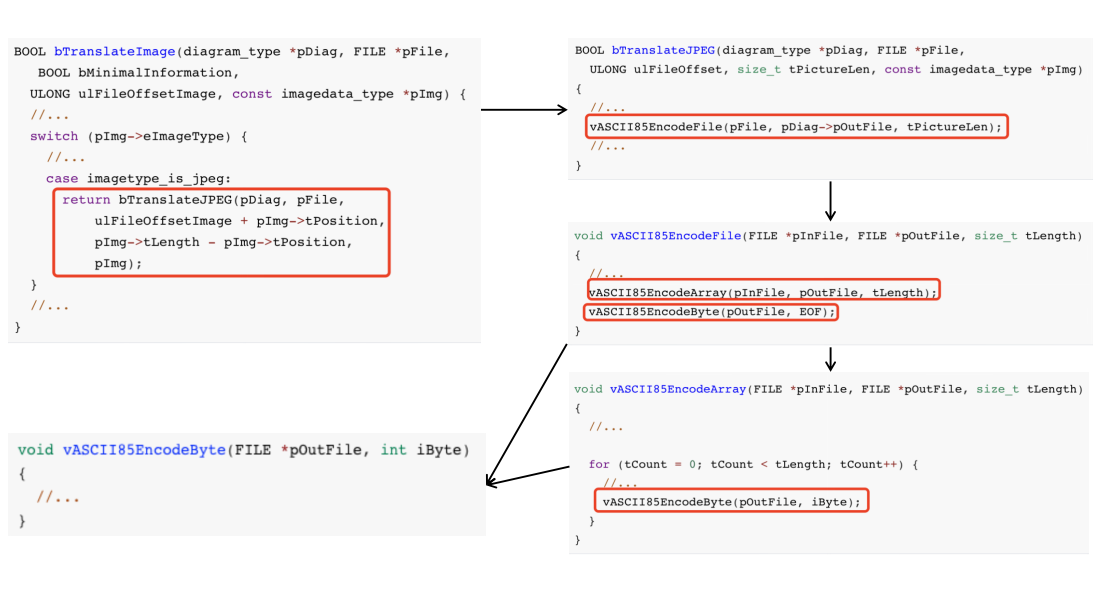
\includegraphics[width = 1\textwidth]{静态分析拒绝样例.jpg}
\caption{依赖闭包方法迭代路径}
\end{figure}

而基于克隆关系的检测方法则更为特殊,其精确率最高,这说明其识别的正例非常准确,很少出现误报。但是它的召回率极低,表明该方法对大部分的变更影响关系无法识别到。这是由于该方法只能识别由于克隆关系产生的变更影响,而在质量良好的项目代码中,克隆代码的现象很少出现,因此提取到样例本身也较少,就导致其整体效果不佳。在实践中,建议基于克隆关系的方法作为其他方法的补充使用。

\textbf{2.针对于RQ2的实验}

RQ1中从整体的角度上说明了三种方法的有效性。为了回答RQ2中三种方法的优势,这里对每种方法检测得到的依赖型和逻辑型的变更影响关系分别进行计算,得到如表的结果。通过对两种类型分别的统计,我们能更直观地发现不同方法的优势和特点。


\begin{table}[htbp]
\caption{变更影响实验结果 - F-measure/召回率/精确度}
\vspace{0.5em}\centering\wuhao
\begin{tabular}{cccccccc}
\toprule
方法 & DB-F-measure & DB-recall & DB-precision & LB-F-measure & LB-recall & LB-precision  \\
\midrule
依赖闭包 & 44.0 & 96.2 & 28.5 & 0 & 0 & 0 \\
克隆代码 & 0 & 0 &  0 & 31.95 & 19.1 & 97.8 \\
历史共现 & 60.3 & 65.9 & 55.6 & 69.3 & 81.7 & 60.2 \\
\bottomrule
\end{tabular}
\end{table}

基于依赖关系闭包方法只能检测依赖型影响关系。其依赖型召回率高达96.2\%,能查全大部分的依赖型影响关系,但准确率不高,导致整体的表现不好。

基于克隆代码的方法仅能检测逻辑型的变更影响关系,但是其准确率能达到95\%。结合RQ1中的分析结果,这表明基于克隆代码方法非常擅长挖掘逻辑型中由于克隆代码导致的变更影响关系。图3-6为克隆代码方法挖掘到的一对有变更影响关系的方法。这里展示了这对方法的部分代码,其中绿色高亮的部分表示代码克隆的区域。这两个方法的主要功能是分别对8位和4位压缩格式的图像进行解码。我们发现,这对方法中的大部分逻辑结构几乎完全相同,只有少部分关键处理逻辑存在差异。由此,我们可以认定,这两个方法的变化过程很可能是同步的,即在实际的维护过程中,当对其中一个方法进行修改时,另一个方法也通常需要同步进行相应的变更,才能保证逻辑的一致性。

\begin{figure}[h]
\centering
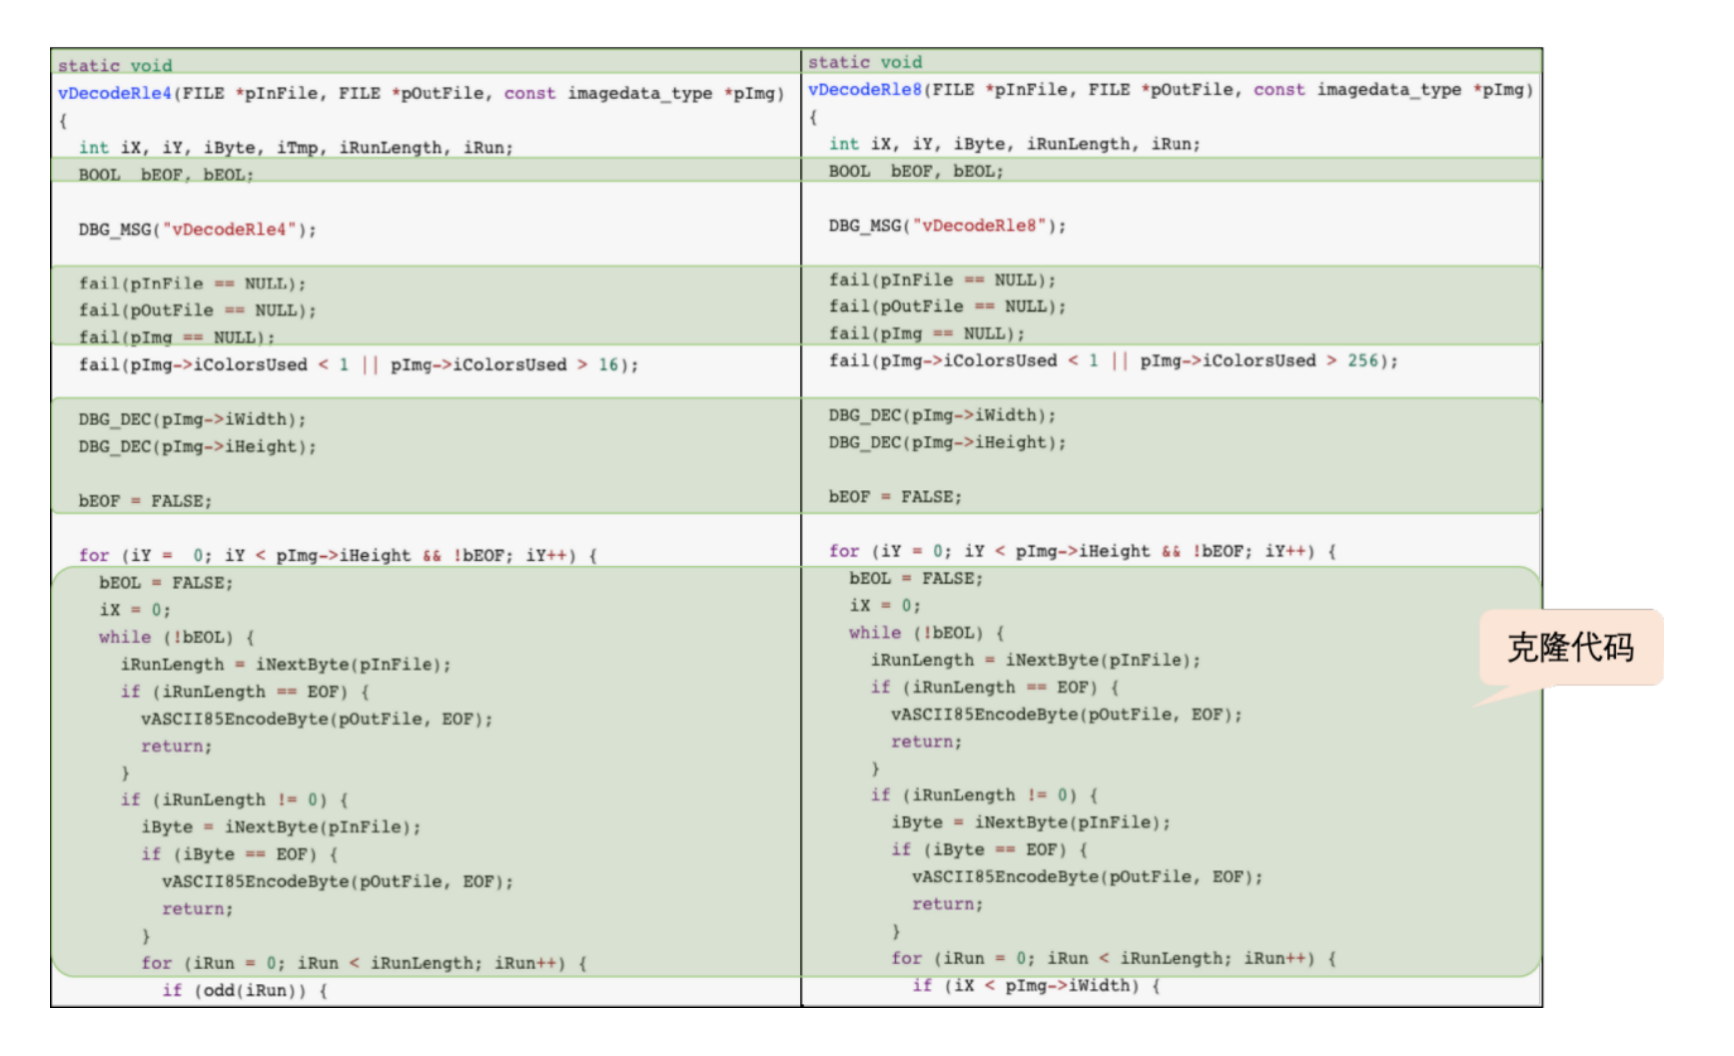
\includegraphics[width = 1\textwidth]{克隆代码示例.jpg}
\caption{包含克隆代码片段的一组方法实例}
\end{figure}

这种代码克隆现象表明,在软件的演化过程中,维护人员可能需要对这两个方法进行联动更新。任何对其中一个方法的修改都可能影响到另一个方法的功能或逻辑一致性,因此在代码维护时,特别是针对这类高度相似的方法,必须考虑它们之间的相互依赖关系。这种潜在的同步更新要求在进行变更影响分析时,尤其是在代码质量评估和变更影响分析的研究中,必须给予充分的关注,以确保系统的稳定性和一致性。

基于数据挖掘的方法可以挖掘两种类型的变更影响关系,根据报告比例,可以发现其报告依赖型更多,这是由于对于质量良好的项目来讲,通常项目中的依赖型变更影响关系更多,能够通过编译器或开发工具即可让开发者掌握项目架构。除此之外该方法对于逻辑型的关系更为擅长,表现为在挖掘到的逻辑型关系中,准确率能达到91.2\%,而对于依赖型的变更影响,则同样存在误报的情况,根据方法的设计思路,推测这里是由于在项目早期,开发者人数较少,项目发展较快,变更较频繁,所以通常都是大量代码一起提交并且频繁更改造成的偶然现象,未来或许可通过仅挖掘项目稳定后的变更历史来改善。

为了说明数据挖掘方法的优秀潜力,以 librdkafka 项目中挖掘到的一对方法为例,该项目是 Apache Kafka 的一个高性能 C/C++ 客户端库。图 3-7 展示了通过数据挖掘技术发现的一对存在变更影响关系的方法。左侧的方法rd\_kafka\_global\_cnt\_decr负责对计数器进行减一操作,而右侧的方法rd\_kafka\_global\_cnt\_incr则负责对计数器进行加一操作。

\begin{figure}[h]
\centering
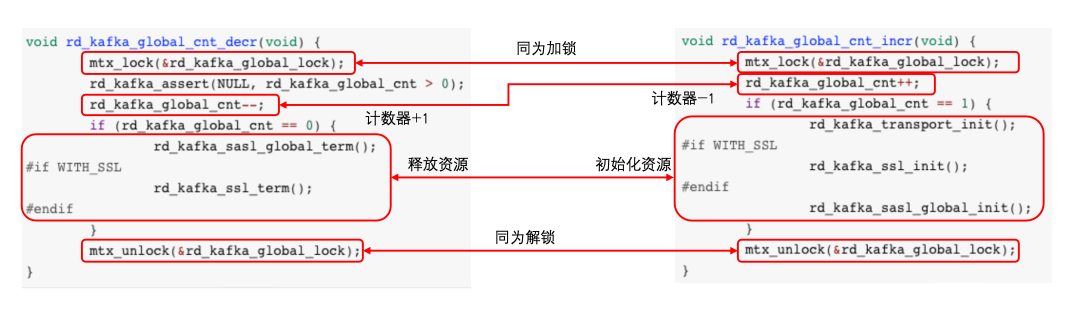
\includegraphics[width = 1\textwidth]{incrdec.jpg}
\caption{逻辑上有变更影响关系的方法对示例-incr和decr}
\end{figure}

从功能上来看,这两个方法是一对典型的协作方法,其作用密切相关。具体来说,incr方法不仅执行计数器加一操作,还在计数器从零变为一时,执行资源的初始化工作,确保所需资源在后续操作中可用。而 decr方法则在计数器减为零时,执行资源的释放操作,以清理不再使用的资源,避免资源泄漏。从代码实现可以看出,这两个方法的操作逻辑具有明显的互补性,加一与减一、初始化与释放的功能关系呈现出“镜像”特性。

尽管它们在代码中并未直接相互调用,也未调用相同的函数,但由于它们在功能上承担了计数器的管理和资源的初始化与释放工作,其逻辑关联性非常强。因此,当其中一个方法的实现逻辑发生变化时,另一个方法通常需要进行相应的调整,以保持整体逻辑的一致性。这种方法对的变更影响关系属于典型的逻辑关联型变更影响关系,而非通过直接调用或共享资源显式连接的变更关系。这种逻辑上的关联性表明,数据挖掘方法能够有效捕获代码中隐性的、非显式的变更依赖。

\begin{figure}[h]
\centering
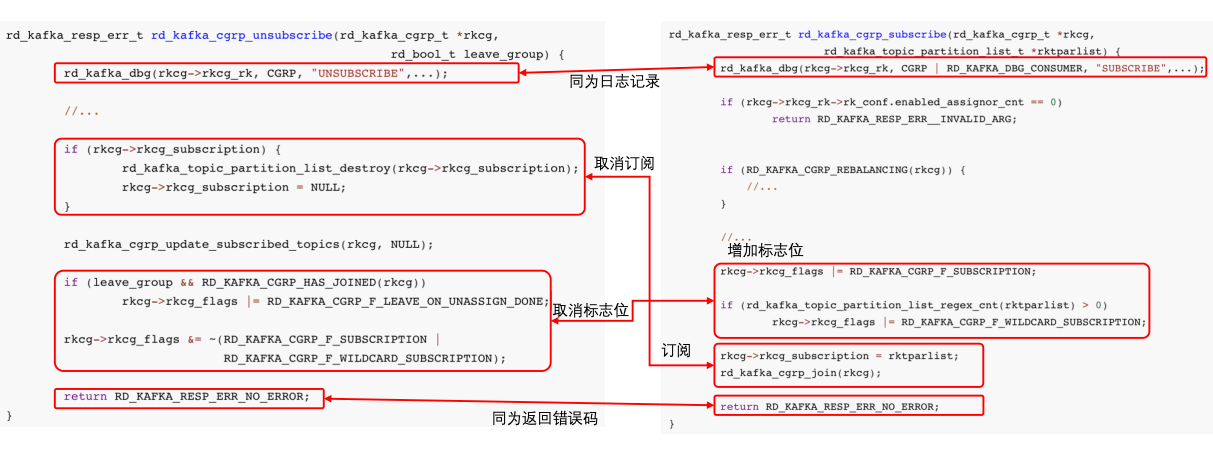
\includegraphics[width = 1\textwidth]{subscribe.jpg}
\caption{逻辑上有变更影响关系的方法对示例-subscribe和unsubscribe}
\end{figure}

图3-8所示是一个更加复杂的例子,这个例子同样是一对有逻辑关联型变更影响关系的方法。这对方法的功能分别是对 Kafka 的主题(topic)进行订阅和取消订阅。左侧的方法负责实现对指定主题的取消订阅操作,而右侧的方法则负责实现订阅操作。尽管这两个方法在代码上并未直接相互调用,但它们在逻辑上具有显著的关联性,尤其是在处理订阅状态的管理上,在订阅操作中,方法会新增订阅标志位、更新订阅的主题列表。而在取消订阅操作中,方法会移除对应的订阅标志位、清空订阅列表,并在必要时清理与订阅相关的组资源。这种逻辑上的互补关系,使得订阅和取消订阅操作形成了一个完整的管理闭环。

从功能视角来看,订阅和取消订阅的行为本质上是对同一资源或逻辑状态的不同操作。这种镜像特性意味着,当订阅逻辑发生变化时,例如新增了订阅标志位的更新规则或修改了主题列表的处理方式,取消订阅逻辑通常也需要进行相应的调整,以保证订阅状态管理的完整性和一致性。

这两对方法体现了典型的逻辑关联型变更影响关系。这种关系不同于通过显式调用或共享资源产生的直接依赖,而是一种通过功能和逻辑流程相互关联的隐性依赖。这种实例表明,即使在方法间没有显式的代码关联,数据挖掘方法仍能够捕获这类隐性逻辑关联,为代码变更影响分析提供了有力支持。通过识别这类方法对,开发者在维护和演化代码时可以更好地理解潜在的影响范围,避免遗漏可能的关联性调整,提高系统维护的可靠性和效率。


\begin{table}[htbp]
    \caption{变更影响实验结果 - F-measure/召回率/精确度}
    \vspace{0.5em}\centering\wuhao
    \begin{tabular}{cccccccc}
    \toprule
    方法 & DB-F-measure & DB-recall & DB-precision & LB-F-measure & LB-recall & LB-precision  \\
    \midrule
    历史共现-2 & 60.3 & 65.9 & 55.6 & 69.3 & 81.7 & 60.2 \\
    历史共现-3 & 63.3 & 54.5 & 75.4 & 76.1 & 69.3 & 84.3 \\
    \bottomrule
    \end{tabular}
    \end{table}
    
    
    本文提出的三种方法均从逻辑型关系的检测上弥补了传统基于依赖传递闭包方法的不足,为代码变更影响关系的检测提供了多样化的解决方案。这些方法各有侧重,适用于不同的应用场景,同时也具有一定的局限性。总结如表3-7。
    
    
    \begin{table}[htbp]
    \caption{变更影响分析方法对比总结}
    \vspace{0.5em}\centering\wuhao
    \begin{tabular}{ccp{4cm}p{4cm}}
    \toprule
    方法& 检测关系 & 适用场景 & 缺点\\
    \midrule
    克隆代码 & 逻辑型中的代码克隆 & 有无代码变更历史均可 & 只能检测代码克隆一种关系\\
    数据挖掘  & 依赖型和逻辑型 & 有代码变更历史的项目 & 无法应用于没有变更历史的项目,如果不频繁变更可能无法被检测 \\
    深度学习  & 依赖型和逻辑型 & 无变更历史的项目 & 依赖于训练数据的质量 \\
    \bottomrule
    \end{tabular}
    \end{table}







\section{本章小结}

本章实现了对代码中间表示的提取及质量评估度量的计算。首先,本文基于 libclang 工具对软件项目进行抽象语法树提取,并在此基础上进一步构建了方法摘要表和全局变量信息表。随后,基于提取得到的中间表示,分别介绍了基于内聚度缺乏度和基于连通性的内聚度分析,介绍了方法间耦合性分析以及扇入扇出的提取和分析,通过这几种分析手段提取了 8 个代码质量指标和 6 种耦合关系。本章通过一系列实验验证了度量指标的有效性,但是发现其只能聚焦于范围较小的质量问题,无法反映软件系统在架构上的缺陷,难以帮助开发者从软件代码的宏观角度上指导软件维护。









% Local Variables:
% TeX-master: "../main"
% TeX-engine: xetex
% End:
